\section{Zielsetzung}

In diesem Versuch sollen die Eigenschaften des Photoeffekts untersucht werden,
also die Frequenzabhängigkeit und Intensitätsunabhängigkeit der Elektronenenergie,
beim Austritt aus von Licht beschienenem Metall.

\section{Theorie}
\label{sec:Theorie}

Der Photostrom, welcher entsteht, wenn Metall mit Licht bestrahlt wird, kann nicht mit dem Wellenbild der klassischen Elektrodynamik erklärt werden.
Hierzu wird von der Korpuskeltheorie ausgegangen, bei der sich die Energie eines Lichtteilchens, eines Photons, über

\begin{equation}
    \label{eqn:photon-energie}
    E_\text{Photon} = h \nu
\end{equation}

berechnet. Dabei ist $h$ das Planck'sche Wirkungsquantum und $\nu$ die Frequenz des Lichtes.


\begin{figure}
  \centering
  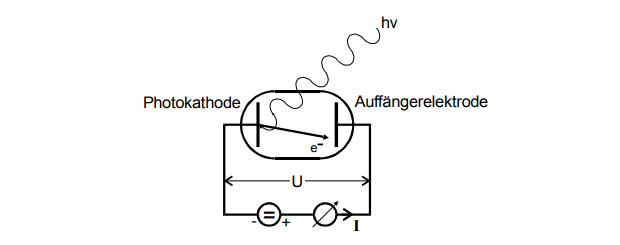
\includegraphics[width=0.95\textwidth]{content/schem-aufbau.png}
  \caption{Schematischer Aufbau der Versuchsapperatur zur Untersuchung des Photoeffekts \cite{V500}.}
  \label{fig:schem-aufbau}
\end{figure}


Zur Untersuchung des Photoeffekts werden zwei Elektroden im Vakuum, wie in \autoref{fig:schem-aufbau} zu sehen, gegenüber gestellt.
Die Photokathode wird anschließend mit monochromatischen Licht bestrahlt.
Dies sorgt dafür, dass sich Elektronen aus dem Material lösen.
Es stellt sich heraus, dass die Elektronenanzahl pro Zeitintervall proportional zu der Intensität des Lichtes und die Elektronenenergie abhängig von der Frequenz des Lichtes ist.

Aus dem Zusammenhang

\begin{equation}
    \label{eqn:elek-energie}
    E_\text{kin} = h \nu - A_\text{k},
\end{equation}

bei dem $A_\text{k}$ die Austrittsarbeit der Elektronen aus dem Material ist,
folgt, dass es eine Mindestfrequenz des Lichtes geben muss, unter der kein Photostrom zu messen ist.
Wenn nun eine beschleunigende Spannung $U$ angelegt wird, sodass

\begin{equation}
    \label{eqn:besch}
    h \nu + e U \geq A_\text{k}
\end{equation}

gilt, kann dennoch ein Strom gemessen werden. Dabei ist $e$ die Elementarladung.

Des Weiteren wird während des Vorgangs ein einzelnes wechselwirkendes Photon vollständig annihiliert.
Seine gesamte Energie wird an ein Elektron übertragen.
Dennoch stellt man fest, dass die kinetische Energie der Elektronen ein kontinuierliches Spektrum ist.
Dies liegt an der Fermi-Dirac-Verteilung im Material selbst. Diese sagt aus,
dass die Elektronen in jenem bereits eine gewisse Energie zwischen $0$ und der Fermie-Energie $\chi$ besitzen,
welche statistisch verteilt ist. Dabei kann $\chi$ einige Elektronenvolt groß sein.

Zur Bestimmung eben jener kinetischen Energie wird die sogenannte Gegenfeldmethode genutzt.
Dazu wird an der Anode eine Gegenspannung $U$ angelegt, welche die Elektronen abbremst.
Diese erreichen die Elektrode nun auschließlich, wenn ihre Energie größer als $e U$ ist.
Also verschwindet der gemessene Strom an der Anode, wenn

\begin{equation}
    \label{eqn:gegenfeld}
    e U = \frac{1}{2} m_\text{e} v_\text{max}^2
\end{equation}

erfüllt ist, wobei $m_\text{e}$ die Elektronenmasse und $v_\text{max}$ die maximale Geschwindigkeit der Elektronen ist.

\begin{figure}
  \centering
  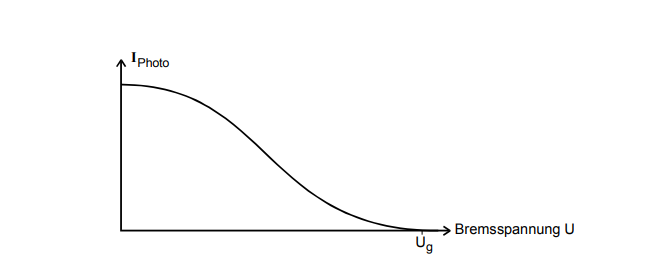
\includegraphics[width=0.95\textwidth]{content/brems-photo.png}
  \caption{Der Photostrom einer mit monochromatischen Licht bestrahlten Photozelle aufgetragen gegen die Bremsspannung \cite{V500}.}
  \label{fig:brems-photo}
\end{figure}

Des Weiteren ist aufgrund der oben erwähnten Fermi-Dirac-Verteilung zu bemerken, dass der Elektronenstrom bei einer bestimmten Spannung $U$ nicht auf 0 abfällt,
sondern sich bereits vorher dieser annähert. Die zu erwartende Kurve ist in \autoref{fig:brems-photo} zu sehen.

Des Weiteren gilt unter bestimmten Voraussetzungen ein parabolischer Zusammenhang zwischen dem Photostrom $I_\text{Ph}$ und $U$:

\begin{equation}
    \label{eqn:i-u}
    I_\text{Ph} \propto U^2.
\end{equation}